%La ventaja para el enfoque jerárquico es que los secuenciadores tienen 
%menos probabilidades de cometer errores al ensamblar los fragmentos 
%``shotgun'' contiguos, mientras sean cromosomas completos. La razón es 
%que la localización cromosómica de cada BAC es conocido, y hay menos
% piezas montadas al azar. La desventaja de este método es tiempo y 
%dinero. El método de la ``shotgun'' es más rápido y menos costoso, pero 
%es más propenso a errores debido a la construcción o montaje de la 
%secuencia final. Por ejemplo, si una porción de 500 kb de un cromosoma 
%se duplica y cada duplicación se corta en fragmentos de 2 KB, entonces
% sería difícil determinar cuando un particular, de 2 piezas kb debe 
%estar ubicado en la secuencia terminada, ya que ocurre dos veces. Se
% podría pensar, "a quién le importa ya que son duplicados? Pero rara 
%vez duplicaciones mantenienen sus secuencias originales, sino que tienden
% a la deriva con el tiempo. Así que una pequeña región se podrá mantener,
% mientras que otras partes pueden mutar. Esto puede crear secuencias de 
%superposición de piezas pequeñas que se encuentran varios cientos de kb 
%de distancia en el cromosoma.
%
%¿Qué método es mejor? Depende del tamaño y la complejidad del genoma.
% Con el genoma humano. Sólo tenemos secuencias de proyecto y cada uno tiene lagunas y 
%regiones sin terminar por lo que no es posible decir con seguridad. 
%Vale la pena mencionar que Celera ha tenido acceso a los datos PGH, pero
% el PGH no tuvo acceso a los datos de Celera. Por otra parte, ya que 
%los datos de Celera no es de libre disposición, la mayoría de los 
%investigadores utilizarán la secuencia de HGP para futuras investigaciones.
% Por lo tanto, nunca puede saber qué método "ganado".


\frame
{
\begin{center}
	\Huge{Comparación}
\end{center}
}

\frame
{
\frametitle{Hierarchical Shotgun vs Shotgun}
\framesubtitle{Principales diferencias}
\begin{center}
	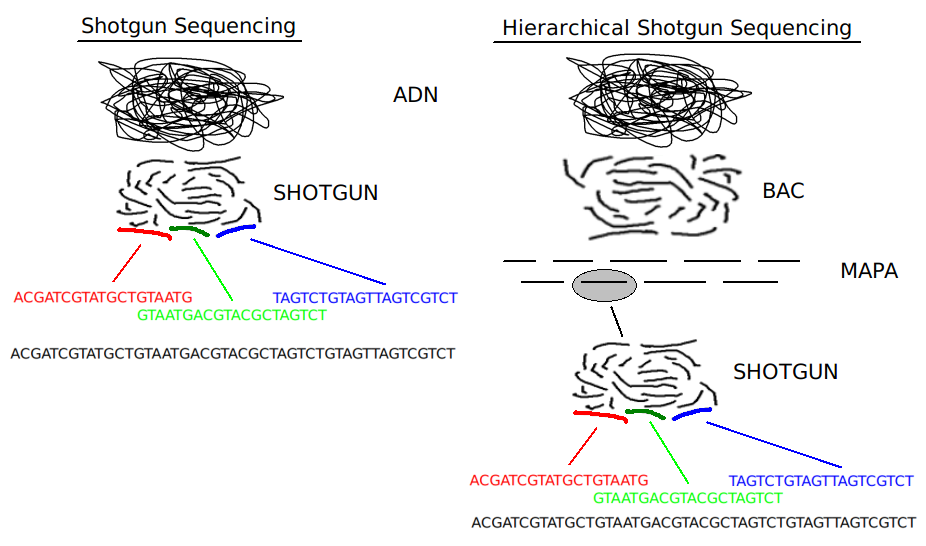
\includegraphics[width=0.9\textwidth]{img/comparacion}
\end{center}
}

\frame
{
\frametitle{Hierarchical Shotgun vs Shotgun}
\framesubtitle{¿Cuál es mejor?}
\begin{itemize}
	\item Depende del tamaño del genoma
	\item Depende de la complejidad del genoma
	\item Depende si se desea exactitud o velocidad.
\end{itemize}
}
